% !TeX root = main.tex
% !TeX encoding = UTF-8
% !TeX spellcheck = <none>

\chapter{LiDAR数据误差分析及处理}

\section{LiDAR数据误差源}

\subsection{量测误差}

\begin{enumerate}
	\item \textbf{测距误差}:激光测距仪是LiDAR系统最重要的核心设备,在所有影响激光脚点坐标精度的因素中,测距精度是最复杂的。
	\begin{enumerate}
		\item {\cukai 测距仪误差}:
		\begin{itemize}
			\item \textit{包括时延估计误差和时间测量误差}。此外还包括传感器激光信号发射与接收不平行(可校正)产生的误差;反光镜的旋转、震动误差;脉冲零点误差等。
			
			此类误差,表现为常数误差,可通过比较利用激光测距和精密测量手段获取同一表面高度的差别来确定,一般在室内测定。
			\item \textit{光学元件引起的误差}
			\begin{itemize}
				\item 背景光反射作用
				\item 光经过光学窗口或被反射镜反射后的衰减
				\item 由光学窗口或反射镜造成的散射(灰尘和光学 元件表面原因)
				\item 经过光学窗口后光速减慢
				\item 光学窗口的曲度造成发射光束和接收光束散焦
			\end{itemize} % 光学元件引起的误差
			\item \textit{探测器影响}
			\begin{itemize}
				\item 一般要求探测器对被探测的光波波长具有最大的响应值,最快的响应速度,由其自身造成的噪声应尽可能小。
				\item 探测器中的噪声包括:信号的出射噪声(shot noise)、暗电流(dark current)噪声,还有热噪声等。
			\end{itemize} % 探测器影响
		\end{itemize} % 测距仪误差
		\item {\cukai 大气损耗引起的误差}:大气改正要同时考虑大气延迟和大气折射,
		一般来讲,每100米激光光程由于大气的影响会产生大约2 cm的距离误差。
		\begin{itemize}
			\item \textit{大气折射影响}:其影响程度取决于激光脉冲的波长;对同一种信号而言,大气折射误差主要与气温、气压和大气湿度有关。
			\item \textit{大气时延影响}:相比GPS载波信号(激光脉冲波长约1微米,GPS载波波长约2分米),激光脉冲信号受此影响较小,绝对量只有几个mm量级。
		\end{itemize} % 大气损耗引起的误差
	\item {\cukai 地物目标引起的误差}
		\begin{itemize}
			\item 由于地表物理特征的不同而产生不同的后向反射
			\begin{itemize}
				\item 如当信号发生漫反射时出现大量反射信号被接收,会形成较大的接收噪声;
				\item 当信号照射到光滑物体表面便形成镜面反射,可能会造成激光测距信号“丢失”;
				\item 另外有的信号可能经几次反射后反射回去,这样测定的时间延迟不能代表真正的时间延迟。
			\end{itemize}
			\item 激光测量精度与还地面粗糙程度、坡度、地物类型等有关。另外,被水域覆盖的地方,红外激光大部分被吸收,只有少量被反射;
			地表不连续以及地物移动,如行人、车辆,动物等都会影响测距的精度。
		\end{itemize} % 地物目标引起的误差
	\end{enumerate} % 测距误差
	\item \textbf{GPS定位误差}:主要包括卫星轨道误差,卫星钟钟差,接收机
	钟钟差,多路径效应,相位中心不稳定,可视
	卫星几何图形强度,观测噪声,整周模糊度求
	解正确与否等。
	\begin{itemize}
		\item 这类误差对定位精度影响较大,且随着观测环境的 变化而不断变化,不容易消除或模型化。
		\item 通常为了削弱GPS定位误差的影响,采用的方法是在测区内建立多个分布较均匀的基准站。
	\end{itemize} %. GPS定位误差
	\item \textbf{IMU姿态误差}:影响定位精度的主要因素之一
	\begin{itemize}
		\item \textbf{主要包括}:
		\begin{itemize*}
			\item 设备安置误差
			\item 加速度计常数误差
			\item 加速度计比例误差
			\item 陀螺仪漂移
			\item 测量噪声
			\item 轴承间的非正交性
			\item 重力模型误差
			\item 大地水准面误差
		\end{itemize*}
		\item \textbf{姿态参量对三维定位精度的影响表现为}:随着飞行高度增加和扫描角度增加姿态量测误差的影响会有所增加。
		\item \textbf{解决办法}:可通过降低飞行高度以减弱INS姿态测量误差对定位的影响。
	\end{itemize} %. IMU姿态误差
	\item \textbf{激光束发散角产生的误差}:由于激光光束都有一定的发散角,与不同的
	目标表面作用时会产生不同程度的脉冲展宽从而增加测
	距的不确定性,使探测信号强度、信噪比与及探测概率
	等呈随机性变化,影响测距仪的测量精度和性能。
	
	对于不同的系统,其影响情况可能有些差异。若LiDAR系统只记录首次回波信号的系统,假设激光光束的发散角为$ \gamma $,那么最大可能带来的角度误差为$ \gamma/2 $,其误差对定位的影响效果类似于扫描角误差。
\end{enumerate} % 量测误差

\subsection{集成误差}
\begin{enumerate}
	\item \textbf{安置误差}
	\begin{enumerate}
		\item {\cukai 偏心距误差}:偏心距误差主要是激光束出射点到IMU系统中心之间的距离以及IMU中心到GPS接收机天线中心的距离的测量误差。
		\item {\cukai 视准轴误差}:视准轴误差指IMU系统与激光测距仪之间的角度安置误差,包括翻滚误差、俯仰误差、航偏误差(图)。
		\begin{figure}[htbp]
			\centering
			\subfloat[翻滚误差]{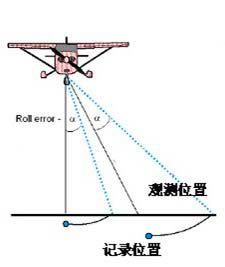
\includegraphics[height=4cm]{figure/Chapter8/翻滚}} \hspace{3em}
			\subfloat[俯仰误差]{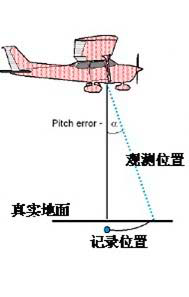
\includegraphics[height=4cm]{figure/Chapter8/俯仰}} \hspace{3em}
			\subfloat[航偏误差]{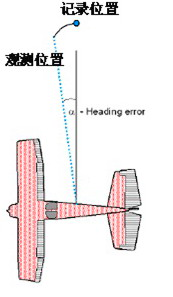
\includegraphics[height=4cm]{figure/Chapter8/航偏}}
			\caption{视准轴误差}
			\label{fig:视准轴误差}
		\end{figure}
		\item {\cukai 扫描角误差}:扫描电机的非匀速扫描以及扫描转镜的震动等引起。
		
		以旋转棱镜为例,如果转镜转速为omega转/秒,扫描视 场范围为$ \theta $弧度,每行采样点数为$ N $,则在以扫描行为单 位的一个周期$ T=1/\omega $中。每个采样点对应的扫描角不是实际量测,而是根据扫描视场范围$ \theta $和每行采样点数计算出来。
		
		因此相应要求扫描电机的匀速旋转,但设计时不能完全保证匀速旋转,从而产生扫描角误差。
		\begin{itemize}
			\item \textit{角度步进误差}:角度记录装置在记录角度变化的时候产生的误差,一般在出厂的时候进行校正 。
			\item \textit{扭矩误差}:扫描镜在旋转和摆动的时候,由于惯性的原因,其转动的实际角度必然会与预期的(记录装置记录的)角度不一样,这就是扭矩误差(图\ref{fig:扭矩误差})
			\begin{figure}
				\centering
				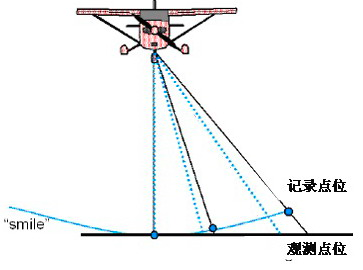
\includegraphics[width=0.4\linewidth]{figure/Chapter8/扭矩误差}
				\caption{扭矩误差}
				\label{fig:扭矩误差}
			\end{figure}
		\end{itemize}
	\end{enumerate} % 安置误差
	\item \textbf{处理误差}
	\begin{enumerate}
		\item {\cukai 时间同步误差}:GPS接收机、INS、激光测距系统独立工作,
		各自的数据采样率不同,即实际数据采样不同步,处理时,需要将它们的时间系统统一到标准UTC(Universal CoordinatedTime)系统。
		
		时间偏差对定位结果的影响会使平坦的表面发生变形或扭曲。
		\item {\cukai 动态时延误差}:如图\ref{fig:动态时延误差示意图}所示,动态时延误差包括两个部分,一部分是由于激光测距和GPS定位数据采集率不同引起的时延改正;另一部分是由于飞机的垂直运动分量引起的附加改正。
		\begin{figure}
			\centering
			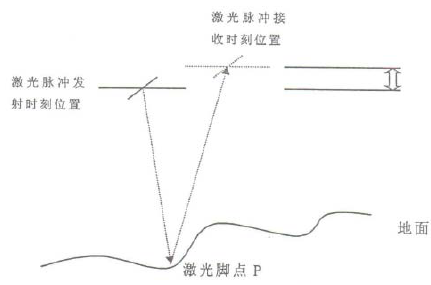
\includegraphics[width=0.4\linewidth]{figure/Chapter8/动态时延误差示意图}
			\caption{动态时延误差示意图}
			\label{fig:动态时延误差示意图}
		\end{figure}
		\item {\cukai 内插误差}:是由于LiDAR各系统具有不同的记录(采样)频率造成的。由于GPS数据采样频率一般为1$ \sim $2Hz;INS数据采样率一般为8$ \sim $50 Hz;而激光扫描测距的脉冲重复频率可达2$ \sim $25 KHz,采样率不一样,最后还要根据采样率低的姿态数据和位置数据内插出每个激光测距记录时刻的姿态和位置,势必产生内插误差。
		\item {\cukai 二类高程误差}:当地面起伏较大或有一定的坡度时,由于激光脚点平面位置的误差而产生的高程方向的附加误差。
		
		假设激光脚点的真实位置(实际不知道)为$ (X_0,Y_0,Z_0) $; 由于受到各种观测误差的影响,由LiDAR推算出的位置为$ (X,Y,Z) $,即
		\begin{equation}
		(X,Y,Z) = (X_0,Y_0,Z_0) + (e_X,e_Y,e_Z)
		\end{equation}
		
		由于平面误差的存在,使得激光脚点的位置由图中的$ (X_0,Y_0,Z_0) $跑到$ (X,Y,Z) $位置,高程误差除了$ e_Z = Z - Z0 $外,还有由平面误差形成的二类高程误差$ e_S $:
		\begin{equation}
		e_S = e_X \tan \varPhi + e_Y \tan \varPsi
		\end{equation}
		\item {\cukai 坐标转换误差}:如图所示。
		\begin{figure}[htbp]
			\centering
			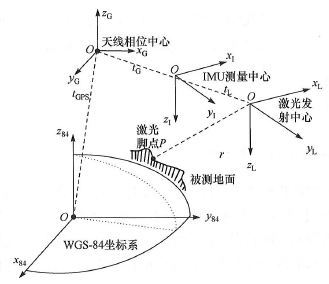
\includegraphics[width=0.4\linewidth]{figure/Chapter8/坐标转换误差}
			\caption{坐标转换误差}
			\label{fig:坐标转换误差}
		\end{figure}
	\end{enumerate} % 处理误差
\end{enumerate} % 集成误差

\section{误差的分析}

\subsection{误差的定性定量分析}

\paragraph{测距误差}测距误差同多种因素有关,包括系统和随机两部分。这里考虑系统误差部分,其大小取决于不同的系统、反射介质及地形条件等外界条件。可用公式表示为
\begin{equation}
\symbf{r}^* = \symbf{r} + ∆\symbf{r} = \begin{pmatrix}
0 \\ 0 \\ \rho + ∆\rho
\end{pmatrix}^{\text{T}}
\end{equation}
式中,$ r^* $是含有测距误差$ ∆\rho $的激光脚点在瞬时激光束坐标系中的位置向量;$ ∆r $为测距误差引起的激光脚点在顺势激光束坐标系中的误差向量。

\paragraph{扫描角误差}会使定义的激光扫描参考坐标系绕X轴旋转一个小角度。同时由于安装时激光扫描平面不可能完全垂直于激光
扫描参考坐标系的X轴,这就使得实际的激光扫描平面绕
扫描参考坐标系的Y轴和Z轴各有一个小的旋转角。因此,
实际坐标变换旋转矩阵为
\begin{equation}
∆\symbf{R}_L = \symbf{R}(∆\kappa)\symbf{R}(∆\varphi)\symbf{R}(∆\tau_i) = 
\begin{pmatrix}
	1         & -∆\kappa & ∆\varphi \\
	∆\kappa   & 1        & -∆\tau_i \\
	-∆\varphi & ∆\tau_i  & 1
\end{pmatrix} 
\end{equation}
因此,激光点在激光扫描坐标系中的坐标为
\begin{equation}
P_L^* = ∆\symbf{\symbf{R}}_L \cdot \symbf{\symbf{R}} \cdot (r + ∆r)
\end{equation}

\paragraph{系统安置误差}激光扫描参考坐标系同惯性平台参考坐标系的坐标轴间不能完全保证相互平行引起的误差。系统安置误差必须经过在航检校测定。旋转矩阵课表示为:
\begin{equation}
∆\symbf{R}_M =
\symbf{R}(∆\gamma)\symbf{R}(∆\beta)\symbf{R}(∆\alpha) = 
\begin{pmatrix}
	1       & -∆\gamma & ∆\beta   \\
	∆\gamma & 1        & -∆\alpha \\
	-∆\beta & ∆\alpha  & 1
\end{pmatrix} 
\end{equation}
偏心改正测定误差包括激光发射参考点在惯性平台参
考坐标系中的分量误差$ ∆t_L $以及GPS天线相位中心在惯性平台参考坐标系中的分量误差$ ∆t_G $两部分。因此对应激光脚点在惯性平台参考坐标系中的坐标为
\begin{equation}
P_M^* = ∆\symbf{R}_M \cdot \symbf{R}_M \cdot ∆\symbf{R}_L \cdot \symbf{R}_L \cdot (\symbf{r} + ∆\symbf{r}) + \symbf{t}_L + ∆\symbf{t}_L - (\symbf{t}_G + ∆\symbf{t}_G)
\end{equation}

\paragraph{姿态测定误差}INS测定姿态角存在误差。假定三个姿态角的测定误
差分别为$ ∆R $、$ ∆P $、$ ∆H $,类似的可以得到误差旋转矩阵
\begin{equation}
∆\symbf{R}_N =
\symbf{R}(∆H)\symbf{R}(∆P)\symbf{R}(∆R) = 
\begin{pmatrix}
	1   & -∆H & ∆P  \\
	∆H  & 1   & -∆R \\
	-∆P & ∆R  & 1
\end{pmatrix} 
\end{equation}
对应激光脚点在当地水平参考坐标系中的坐标为:
\begin{equation}
P_{\text{LH}}^* = ∆\symbf{R}_N \cdot \symbf{R}_N \cdot (∆\symbf{R}_M \cdot \symbf{R}_M \cdot ∆\symbf{R}_L \cdot \symbf{R}_L \cdot (\symbf{r} + ∆\symbf{r}) + \symbf{t}_L + ∆\symbf{t}_L - (\symbf{t}_G + ∆\symbf{t}_G))
\end{equation}

\paragraph{GPS定位误差}GPS动态差分定位过程中,会受到包括对流层延迟误差、电离层延迟误差、多路径误差等系统误差的影响。若用$ \text{\bfseries APC}_w $表示GPS定位模型,则激光点的几何模型可表示为
\begin{equation}
P_W^* = \symbf{R}_W \cdot \symbf{R}_G \cdot ∆\symbf{R}_N \cdot \symbf{R}_N \cdot (∆\symbf{R}_M \cdot \symbf{R}_M \cdot ∆\symbf{R}_L \cdot \symbf{R}_L \cdot (\symbf{r} + ∆\symbf{r}) + \symbf{t}_L + ∆\symbf{t}_L - (\symbf{t}_G + ∆\symbf{t}_G)) + \text{\bfseries APC}_W + ∆\text{\bfseries APC}_W
\end{equation}

\paragraph{时间偏差}时间偏差主要包括同步误差和内插误差,当同步误差
<10$ \sim $4 sec就不会带来位置误差,同步误差和内插误差表现为随
机特性。

含有各项误差影响的LiDAR几何模型可表示如下:
\begin{equation}\label{equ:含有各项误差影响的LiDAR几何模型}
P_W^* = \symbf{R}_W \cdot \symbf{R}_G \cdot ∆\symbf{R}_N \cdot \symbf{R}_N \cdot (∆\symbf{R}_M \cdot \symbf{R}_M \cdot ∆\symbf{R}_L \cdot \symbf{R}_L \cdot (\symbf{r} + ∆\symbf{r}) + \symbf{t}_L + ∆\symbf{t}_L - (\symbf{t}_G + ∆\symbf{t}_G)) + \text{\bfseries APC}_W + ∆\text{\bfseries APC}_W + ∆t_{\text{TB}}
\end{equation}

\subsection{误差整体分析}

\paragraph{LiDAR点云定位方程}根据激光测距数据、激光器位置的GPS量测数据及姿态数据计算地面点三维坐标的公式。

\paragraph{通用构像方程}设地面点$ P $在地面坐标系中
的坐标为$ (X,Y,Z)_P $,$ P $在传感器坐标系中的坐标
为$ (U,V,W)_P $,投影中心$ G $在地面坐标系中
的坐标为$ (X,Y,Z)_G $,则$ P $点的地面坐标可用通用构像方程表示
\begin{equation}
\begin{pmatrix}
X \\ Y \\ Z
\end{pmatrix}_P = \begin{pmatrix}
X \\ Y \\ Z
\end{pmatrix}_G + \symbf{A} \begin{pmatrix}
U \\ V \\ W
\end{pmatrix}_P
\end{equation}
其中,$ \symbf{A} $为旋转矩阵。

\paragraph{线扫描误差的影响}
\begin{itemize}
	\item GPS的定位误差与激光测距点的定位误差关系
		是$ 1:1 $的关系,而且仅在同一方向上产生影响,
		即激光测距点X坐标的误差只与GPS定位误差中
		$ X $方向上的误差有关,$ Y $、$ Z $方向也是如此。
	\item 各项系数随扫描角及测距数据的变化而变化
	\item 在同一扫描线上,不同测距点上坐标的精度不同;
		对于不同扫描线,各项系数具有一定周期性变化
		的特点。
\end{itemize}

\paragraph{总结}
\begin{itemize}
	\item 在GPS定位精度、姿态量测精度、激光测距精度
		和码盘测量扫描角精度等保持不变的情况下,\textbf{同一条扫描线上不同位置的定位精度是不同的},
		圆锥扫描也是这样,扫描角不同,定位精度也有差异。
	\item \textbf{圆锥扫描方式总体性能比线扫描方式好},其定
		位误差小,定位误差的变化幅度也小,\textbf{这说明采用圆锥扫描方式,激光脉冲的利用率大大提高},
		缩小了激光测距点的间距,增加了单位面积内激光测距点的密
		度,对提高激光点定位精度是非常有利的。
	\item \textbf{对于线扫描方式},随着扫描角的增加,定位精度
		下降,扫描方向($ Y $方向)误差比飞行方向和$ Z $方向误
		差要大,\textbf{这主要是由于测量扫描角的码盘的量测误差引起的},
		这可以从有关误差传播分析的公式中反映出来,
		飞行方向的定位精度则几乎不受码盘量测精度的
		影响。
	\item \textbf{对于圆锥扫描方式来说,主要是$ Z $方向的误差,这个误差比$ X $方向和$ Y $方向要大},
		GPS定位精度、激光测距精度、
		姿态量测精度和码盘测角精度逐次下降情
		况下的定位精度反映了圆锥扫描方式定位精度的总体
		趋势,只要能保证上述四种量测精度,就可以达到很
		好的效果。
	\item \textbf{集成系统}在数据处理的各个环节上都会产生一
		些误差,主要包括激光测距误差、扫描角误差、GPS
		定位误差、IMU姿态误差、部件集成安置误差等。因
		此,采取一定的方法减小误差,提高精度,成为激光
		遥感集成系统工程的关键问题。
\end{itemize}

\section{误差处理}
\subsection{LiDAR误差检测及消除}
根据误差来源分析,机载LiDAR系统受到多种误
差源的影响,为了提高机载LiDAR的精度,最大
可能地降低各种系统误差的影响,一般有三种方
法:
\begin{itemize}
	\item 建立误差改正模型
	\item 仪器检校
	\item 条带平差改正
\end{itemize}

\subsubsection{建立误差改正模型}
有些系统误差可以建立误差模型进行消除。比
如激光脉冲在大气中的传播延迟误差;前面讨
论的二类高程误差;GPS动态定位中的相关误
差源等。

\subsubsection{检校}
\paragraph{检校的原则}
\begin{itemize}
	\item 有些系统误差能够单独检校出来,而有些系统误差彼此相关,难以分离。
	\item 对于不同的扫描方式,检校方法会有些差异。
	\item 一般在讨论其中一种误差源的影响时,认为不受其它误差源的影响,或忽略其它误差的影响。
	\item 而在实际飞行过程,这些误差是相互相关的,所有误差对最后坐标的影响并不是各项的简单叠加,而应该根据式\eqref{equ:含有各项误差影响的LiDAR几何模型}计算。
\end{itemize}

\paragraph{检校的两种状态}
\begin{enumerate}
	\item {\cukai 静态检校}比较容易分析。假设系统安置在直升飞机上,飞机停在一个升降台上,提升升降台 进行静态扫描测量。当扫描角$ \theta=0 $时,激光脚点坐标高程分量只受到测距误差和偏心元素 测定误差的影响。此时有
		\begin{equation}
		e_0^Z = ∆\rho_i + \delta Z_{\text{LG}}
		\end{equation}
		当扫描角分别取得最大值和最小值时,也就是对应于扫描线的两端,根据公式可得扫描线最左端高程$ Z_L $和最右端高程$ Z_R $值,两者之差就有
		\begin{equation}
		Z_L - Z_R = 2H ∆\alpha \tan \theta_{\max}
		\end{equation}
		可求解出其中一个视准轴误差$ ∆a $。
		\begin{itemize}
			\item \textbf{优点}:不受姿态测定误差和GPS动态定位误差的影响。
			\item \textbf{缺点}:不一定适合实际工作时误差影响的情形。
		\end{itemize}
	\item {\cukai 动态检校}比较多见。
\end{enumerate}

\paragraph{视准轴误差的检校}
性能优良的GPS/INS组合定位定姿系统为获取载体高精度的位置、姿态参数提供支持,这是机载LiDAR实 现高精度对地定位的前提。
但由于激光扫描三个主轴与载体坐标系的三个主轴不相互平行,会产生视准轴误差。
直接测定比较困难,通常都是利用自行检校技术直接从机载LiDAR数据中估计出视准轴误差。
视准轴误差是机载LiDAR中最大的系统误差源,根据经验观测这些安置角误差通常为0.1$ \sim $0.3°,这些安置角误差对地面激光脚点坐标的影响还取决于飞行的高度和扫描角的大小,有必要进行消除。
\begin{enumerate}
	\item {\cukai 视准轴误差手工检校方法}
		\begin{itemize}
			\item \textbf{检校顺序}:翻滚误差检校→俯仰误差检校→航偏误差检校
			\item \textbf{翻滚误差的检校}:翻滚误差会造成航带的倾斜(一边高,一边低,图\ref{fig:翻滚误差对航带的影响}),在设计航线的时候,为了使相邻航带间的翻滚误差最大(最明显,容易修正),\textbf{需要使用相同的航高,沿着相对的方向各飞行一条航带}。如图\ref{fig:侧滚角的计算}所示,翻滚的大小为
				\begin{equation}
				\text{Roll}_ω = \arctan \dfrac{∆h / 2}{r}
				\end{equation}
				式中,$ ∆h $为相同飞行高度条件下相向飞行的两条航带间近似同名点的高程差;$ r $为近似同名点到航带中心的垂直距离。
			\item \textbf{俯仰误差的检校}:如图\ref{fig:俯仰误差对航带的影响}所示。俯仰误差的大小与航高相关,在同一航高时,误差的表现在数据难以辨别。\textbf{需要使用不同航高的相对飞行的相邻航带}数据才能看出其误差。如图\ref{fig:俯仰角的计算}所示,俯仰角的大小
				\begin{equation}
				\text{Pitch}_φ = \arccos\dfrac{∆H}{∆H + ∆h}
				\end{equation}
				式中,$ ∆H $与$ ∆h $分别为航高差与同名点计算得到的高程差。
			\item \textbf{航偏误差的检校}:如图\ref{fig:航偏误差对航带的影响}所示,航偏误差与飞行的方向是无关的,使用相对飞行的航线无法判读航偏误差。其检校的方法是使用相互垂直(同一航高即可)的两条航线,在重叠区域内,航偏误差会达到最大,可以比较容易判别。需选取十字飞行的两个条带,在其中一条的中心位置和另一条的边缘重叠区内,寻找尖顶房或坡面,量测平均分离值$ ∆x $和到条带中心的距离$ ∆r $,航偏角的大小为
				\begin{equation}
				\text{Heading}_κ = \arctan \dfrac{∆x}{∆r}
				\end{equation}
		\end{itemize}
		\begin{figure}[htbp]
			\centering
			\subfloat[翻滚误差对航带的影响]{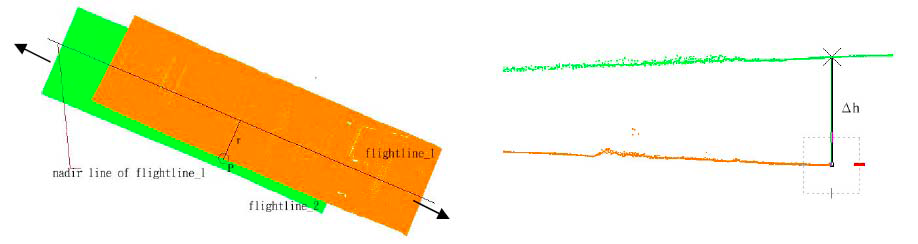
\includegraphics[height=2.5cm]{figure/Chapter8/翻滚误差对航带的影响}\label{fig:翻滚误差对航带的影响}}\\
			\subfloat[俯仰误差对航带的影响]{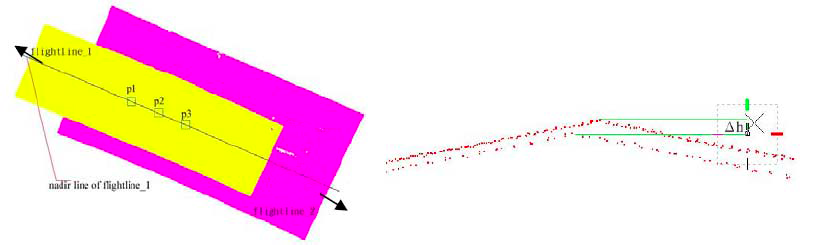
\includegraphics[height=2.5cm]{figure/Chapter8/俯仰误差对航带的影响}\label{fig:俯仰误差对航带的影响}} \hfill
			\subfloat[航偏误差对航带的影响]{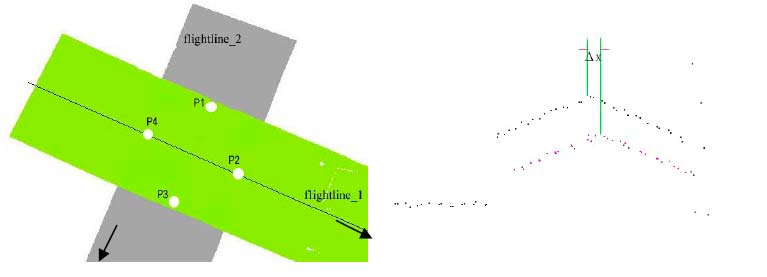
\includegraphics[height=2.5cm]{figure/Chapter8/航偏误差对航带的影响}\label{fig:航偏误差对航带的影响}}
			\caption{视准轴误差对航带的影响}
			\label{fig:视准轴误差对航带的影响}
		\end{figure}
		\begin{figure}[htbp]
			\centering
			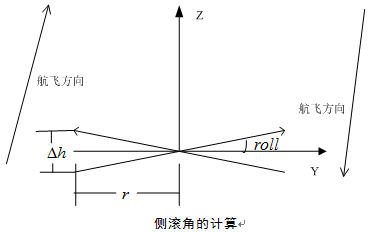
\includegraphics[width=0.4\linewidth]{figure/Chapter8/侧滚角的计算}
			\caption{侧滚角的计算}
			\label{fig:侧滚角的计算}
		\end{figure}
		\begin{figure}[htbp]
			\centering
			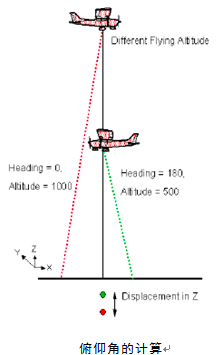
\includegraphics[width=0.3\linewidth]{figure/Chapter8/俯仰角的计算}
			\caption{俯仰角的计算}
			\label{fig:俯仰角的计算}
		\end{figure}
	\item {\cukai 一种无需检校飞行的视准轴误差检校方法}
		\begin{itemize}
			\item \textbf{顺序}:翻滚误差检校→航偏误差检校→俯仰误差检校。首先消除翻滚造成的同名地物高程差异; 然后在用同向航线检校航偏以消除其反向航向上的影响;最后用反向航向检校俯仰。
			\item \textbf{对飞行行线的要求}:如图\ref{fig:无需检校飞行的视准轴误差检校方法对航线的要求}b所示。
				\begin{itemize}
					\item 为能够使用测区航线进行视准轴检校,只需每架次航飞时选择一条航线进行“跳线”飞行。
					\item 测区必须要有复合条件的人字形屋顶类的建筑物存在。
				\end{itemize}
				\begin{figure}[htbp]
					\centering
					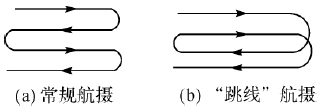
\includegraphics[width=0.3\linewidth]{figure/Chapter8/无需检校飞行的视准轴误差检校方法对航线的要求}
					\caption{无需检校飞行的视准轴误差检校方法对航线的要求}
					\label{fig:无需检校飞行的视准轴误差检校方法对航线的要求}
				\end{figure}
			\item \textbf{翻滚检校}:如果没有飞行检校场数据,仅利用相邻航带的重叠区域进行检校时,由于视准轴系统偏差很微小,且相邻航线旁向重叠距离有限,图中所示相邻航线反向时(航线$ B $和$ C $),翻滚的表现并不明显,重叠区域断面点云基本上难以看到交叉。
			
			如图\ref{fig:翻滚角的影响},利用同向两个条带数据则能够准确测算翻滚视准轴偏差值
			\begin{equation}
			\text{Roll}_ω = \arctan \dfrac{S}{L-D}
			\end{equation}
			其中,$ S $为高程差值,$ L $为测量点位置的激光条带宽度,$ D $为测量位置的两相邻条带重叠部分的宽度。
			\item \textbf{俯仰检校}:如图\ref{fig:俯仰角的影响},利用测区两个相邻但航向相反的条带,选择重叠区域内的尖顶房屋(房屋的屋脊线应垂直于航向),通过沿航向的断面能够量算尖顶的偏移值,从而测算存在的俯仰值
			\begin{equation}
			\text{Pitch}_φ = \arccos \dfrac{D}{2H}
			\end{equation}
			其中,$ D $为量测的尖顶分离值;$ H $为平均相对航高。
			\item \textbf{航偏检校}:如图\ref{fig:旋偏角的影响},在同向飞行的两条相邻航线的重叠部分选取区域内尖顶房屋(屋脊线应垂直于航向),通过测量尖顶偏移值进而计算航偏值
			\begin{equation}
			\text{Heading}_κ = \arcsin \dfrac{S}{L}
			\end{equation}
			其中,$ S $为测量的尖顶房屋分离值;$ L $为相邻航线中心线间距离。
		\end{itemize}
		\begin{figure}[htbp]
			\centering
			\subfloat{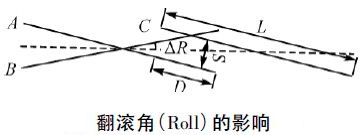
\includegraphics[height=2.5cm]{figure/Chapter8/翻滚角的影响}\label{fig:翻滚角的影响}}\hspace{3em}
			\subfloat{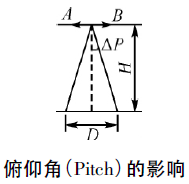
\includegraphics[height=2.5cm]{figure/Chapter8/俯仰角的影响}\label{fig:俯仰角的影响}}\hspace{3em}
			\subfloat{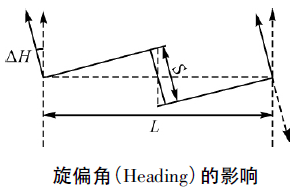
\includegraphics[height=2.5cm]{figure/Chapter8/旋偏角的影响}\label{fig:旋偏角的影响}}
			\caption{无需检校飞行的视准轴误差检校中视准轴误差的影响}
			\label{fig:无需检校飞行的视准轴误差检校中视准轴误差的影响}
		\end{figure}
\end{enumerate}

\subsubsection{条带平差改正}

\paragraph{原理}
如图\ref{fig:系统检校典型飞行航线}所示,如果激光光束的空间方位有误差,不同航带测定
的同一点的坐标和高程间就彼此会有差异,可以
利用多条航带的重叠区域数据进行改正。
\begin{figure}[htbp]
	\centering
	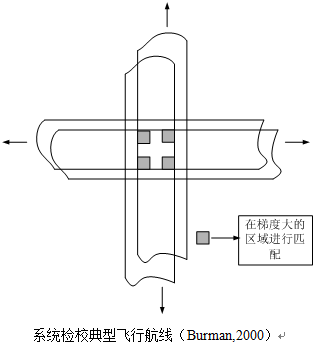
\includegraphics[width=0.4\linewidth]{figure/Chapter8/系统检校典型飞行航线}
	\caption{系统检校典型飞行航线}
	\label{fig:系统检校典型飞行航线}
\end{figure}


\paragraph{方法}
根据这些差异建立相应的参数模型,利用一定的
匹配技术将不同的航带的条带重叠部分联系起来
,通过最小二乘平差,求解这些参数。然后利用
求解出的参数改正每条航带的激光脚点坐标。

\paragraph{难点}
重叠区域激光“同名点” 的匹配,一般都是找重叠区域的地物的特征点作
为联系点。

\paragraph{效果}如图\ref{fig:条带平差改正效果}所示。
\begin{figure}[htbp]
	\centering
	\subfloat{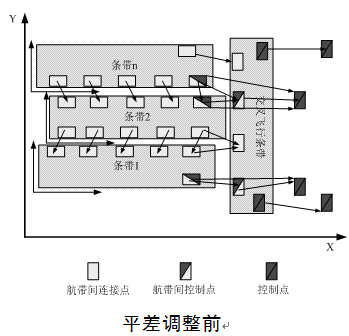
\includegraphics[height=6cm]{figure/Chapter8/平差调整前}}
	\subfloat{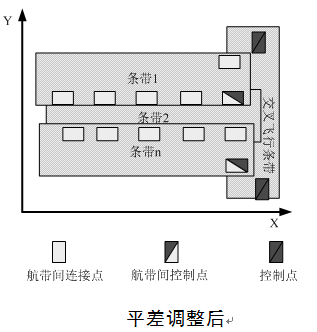
\includegraphics[height=6cm]{figure/Chapter8/平差调整后}}
	\caption{条带平差改正效果}
	\label{fig:条带平差改正效果}
\end{figure}

\subsection{LiDAR工程实践中的误差分析及处理}
\subsubsection{误差分析}

\begin{multicols}{2}
	\begin{enumerate}
		\item \textbf{飞行计划}
			\begin{itemize}
				\item 与地面参考站距离
				\item 参考站的数量及分布
				\item 飞行高度
				\item 扫描角度
			\end{itemize}
		\item \textbf{系统集成}
			\begin{itemize}
				\item 同步误差
				\item 偏心量测误差
				\item IMU和Laser的角度偏差(视准轴误差)
			\end{itemize}
		\item \textbf{专门设备}
			\begin{enumerate}
				\item {\cukai GPS误差}
					\begin{itemize}
						\item 相位测定不准确
						\item 大气延时
						\item 太阳活动干扰
						\item 其它随机误差
					\end{itemize}
				\item {\cukai IMU误差}
					\begin{itemize}
						\item 安置误差:\begin{itemize*}\item 水平 \item 陀螺仪位置 \end{itemize*}
						\item 漂移
						\item 量测噪声
						\item 坐标轴不互相垂直
						\item 加速度计测量误差
					\end{itemize}
				\item {\cukai 激光测距仪}
					\begin{itemize}
						\item 激光脚点的随机抖动
						\item 测距的漂移偏差
						\item 测距误差
						\item 角度量测误差
						\item 其他不明原因引起的误差
					\end{itemize}
			\end{enumerate}
		\item {\cukai 处理过程}
			\begin{itemize}
				\item 坐标转换误差
				\item 水准面校正误差
				\item 滤波处理误差
				\item 地物提取误差
			\end{itemize}
	\end{enumerate}
\end{multicols}

\subsubsection{误差评估}

\paragraph{误差评估的方法}
\begin{itemize}
	\item 可视化检查
	\item 航带叠加分析
	\item 与参考高程数据比较
	\item 与现有地图数据比较
\end{itemize}

\paragraph{可视化检查}将测区内各航带的数据同时加载,叠加影像。
\begin{enumerate}
	\item \textbf{系统误差}:系统误差引起的高程差异和强度差异。
	\item \textbf{滤波算法质量}
	\item \textbf{地物提取质量}:如图\ref{fig:地物提取质量}。
\end{enumerate}
\begin{figure}[htbp]
	\centering
	\subfloat[地物提取误差]{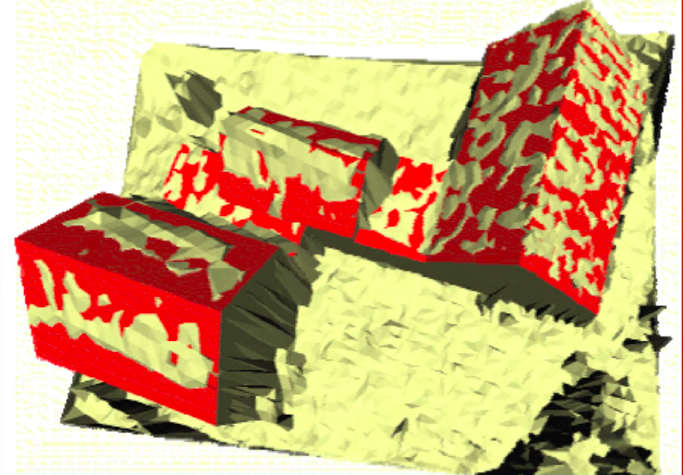
\includegraphics[height=4cm]{figure/Chapter8/地物提取误差}}\hspace{3em}
	\subfloat[点云造成的重建误差]{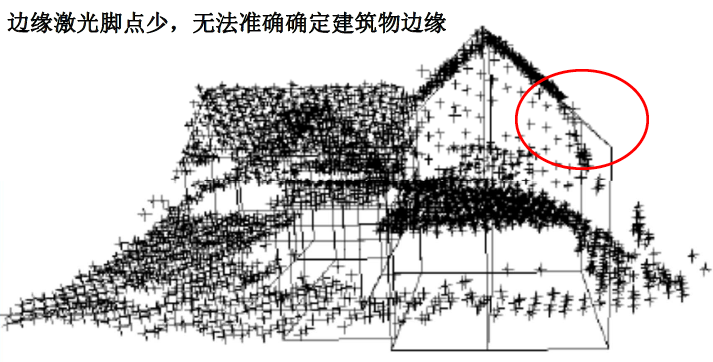
\includegraphics[height=4cm]{figure/Chapter8/点云造成的重建误差}}
	\caption{地物提取质量}
	\label{fig:地物提取质量}
\end{figure}

\paragraph{航带叠加分析}
\begin{enumerate}
	\item \textbf{作用}:
		\begin{itemize}
			\item 可以估算出LiDAR的量测误差
			\item 分析误差的来源
			\item 可辅助航带校正
		\end{itemize}
	\item \textbf{高程误差估算}:选择平坦地区,利用航带重叠处点云进行剖面高程统计分析,估算出高程误差,如图\ref{fig:高程误差估算原理}所示。
	
		•\textbf{不同扫描线之间的差异}:
		\begin{itemize}
			\item 将奇数和偶数扫描线分开,分别生成DEM,如图\ref{fig:测区DEM}。
			\item 两者相减,以颜色表示差别,如图\ref{fig:奇数和偶数扫描线的差异}。
			\item \textbf{原因}:正多面体棱镜的边长有差异。
		\end{itemize}
		\begin{figure}[htbp]
			\centering
			\subfloat[高程误差估算]{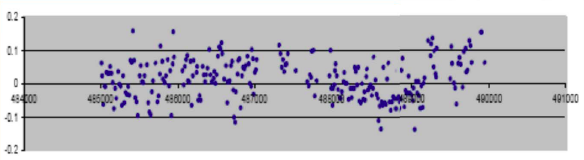
\includegraphics[width=0.5\linewidth,height=3cm]{figure/Chapter8/高程误差估算}\label{fig:高程误差估算原理}}
			\subfloat[测区DEM]{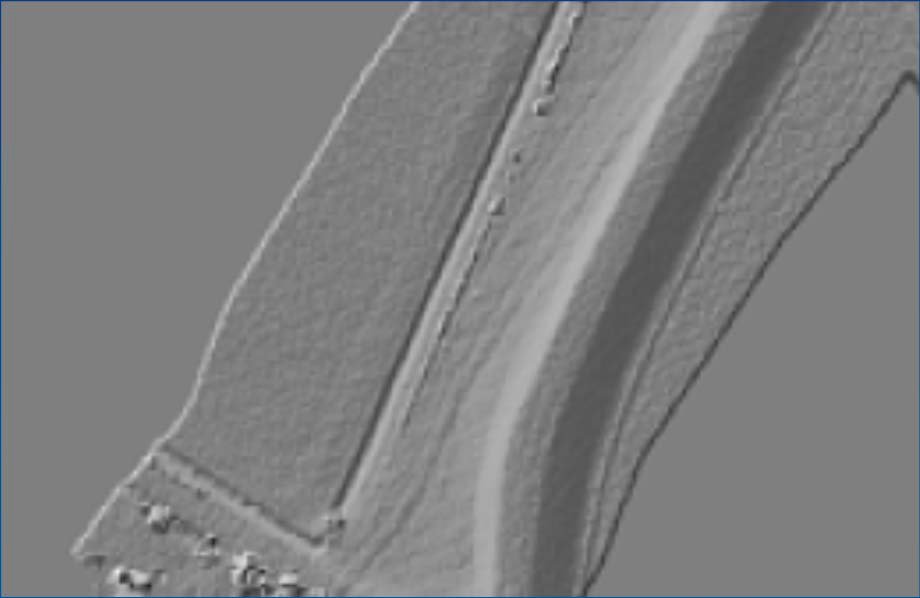
\includegraphics[height=3cm]{figure/Chapter8/测区DEM}\label{fig:测区DEM}}
			\subfloat[奇数和偶数扫描线的差异]{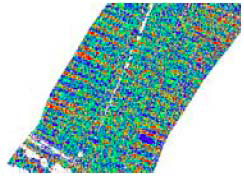
\includegraphics[height=3cm]{figure/Chapter8/奇数和偶数扫描线的差异}\label{fig:奇数和偶数扫描线的差异}}
			\caption{高程误差估算}
			\label{fig:高程误差估算}
		\end{figure}
	\item \textbf{航带间平面位置漂移}:
		\begin{enumerate}
			\item \textbf{原因}:IMU安置误差、GPS误差、仪器标定误差
			\item \textbf{表现形式}:相邻航带同一地物的平面位置及高程的不一致。
			\item \textbf{平面漂移的估计}:
				\begin{itemize}
					\item \textbf{可通过均匀的倾斜地面估计}(如图\ref{fig:通过均匀倾斜地面估计1}、图\ref{fig:通过均匀倾斜地面估计2}),
						但仅依据高程差异判断是不充分的(图\ref{fig:通过均匀倾斜地面估计问题})。
					\item \textbf{使用强度图像}
						\begin{itemize}
							\item 噪声太大
							\item 若质量够好,应选择具有较长边缘作为校正的参照。
						\end{itemize}
					\item \textbf{估计方法}
						\begin{itemize}
							\item 首先进行强度图像内插,然后基于影像匹配技术进行同名特征匹配;
							\item 以同名点作为控制点,求出漂移系数
								\begin{align}
									\begin{split}
										X_S          & = X_t + ∆X          \\
										Y_S          & = Y_t + ∆Y          \\
										Z_S(X_S,Y_S) & = Z_t(X_t,Y_t) + ∆Z
									\end{split}
								\end{align}
						\end{itemize}
				\end{itemize}
		\end{enumerate}
		\begin{figure}[htbp]
			\centering
			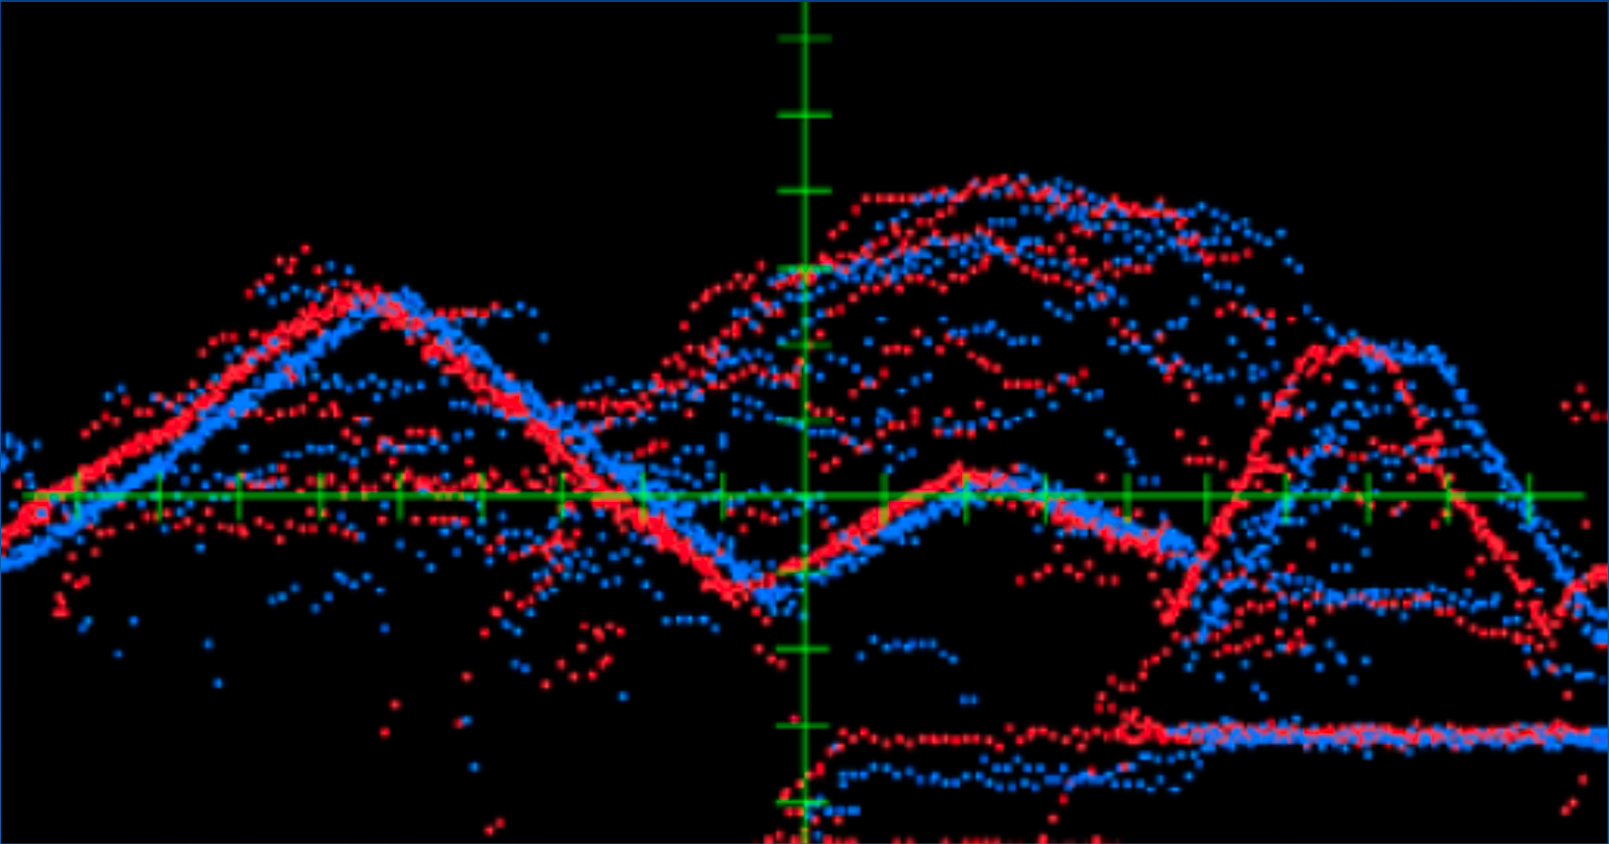
\includegraphics[width=0.5\linewidth]{figure/Chapter8/航带间平面位置漂移}
			\caption{航带间平面位置漂移}
			\label{fig:航带间平面位置漂移}
		\end{figure}
		\begin{figure}[htbp]
			\centering
			\subfloat[]{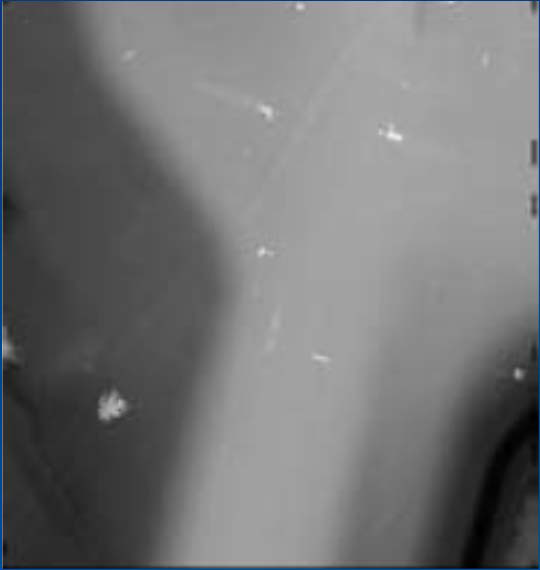
\includegraphics[height=3cm]{figure/Chapter8/通过均匀倾斜地面估计1}\label{fig:通过均匀倾斜地面估计1}}\hspace{3em}
			\subfloat[]{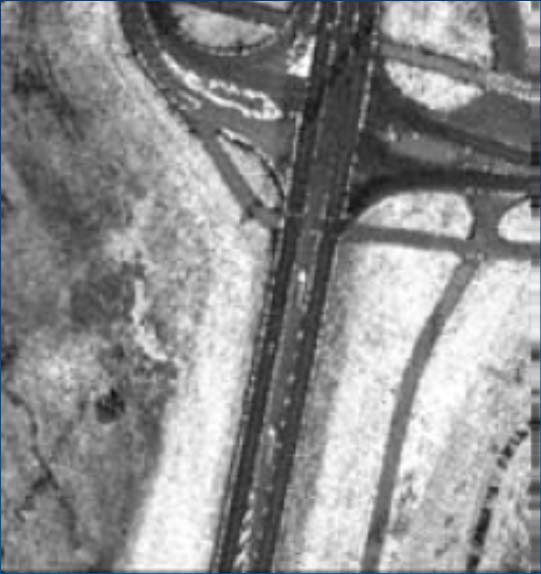
\includegraphics[height=3cm]{figure/Chapter8/通过均匀倾斜地面估计2}\label{fig:通过均匀倾斜地面估计2}}\hspace{3em}
			\subfloat[]{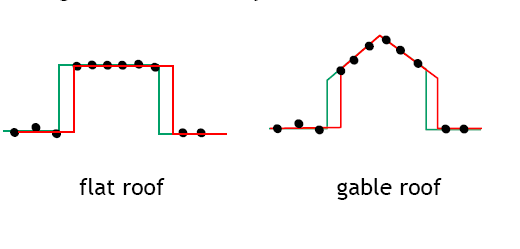
\includegraphics[height=3cm]{figure/Chapter8/通过均匀倾斜地面估计问题}\label{fig:通过均匀倾斜地面估计问题}}
			\caption{通过均匀倾斜地面估计平面漂移}
			\label{fig:通过均匀倾斜地面估计平面漂移}
		\end{figure}
	\item \textbf{同名点查找的数据集格式}
		\begin{itemize}
			\item \textbf{规则格网}:\begin{itemize*} \item 运行速度快 \item 很多主流软件平台支持 \item 内插误差较大 \end{itemize*}
			\item \textbf{三角网}:\begin{itemize*} \item 精度较高 \item 对程序的性能要求较高 \end{itemize*}
			\item \textbf{高程漂移估计}:通常采用拟合方法进行估计,可以避免栅格数据的内插误差,也可以避免强度数据受噪声影响,以及难以获取均匀的倾斜地面等因素造成的匹配误差。
			
			\textbf{拟合区域选择为}:\begin{itemize*} \item 沟渠 \item 人字形屋顶 \end{itemize*}
		\end{itemize}
\end{enumerate}

\paragraph{参照现有高程数据}现有高程数据是摄影测量方法获得的数据或地面测量方法得到的数据,可以评估滤波算法的误差,如图\ref{fig:参照现有的高程数据}所示。
\begin{figure}[htbp]
	\centering
	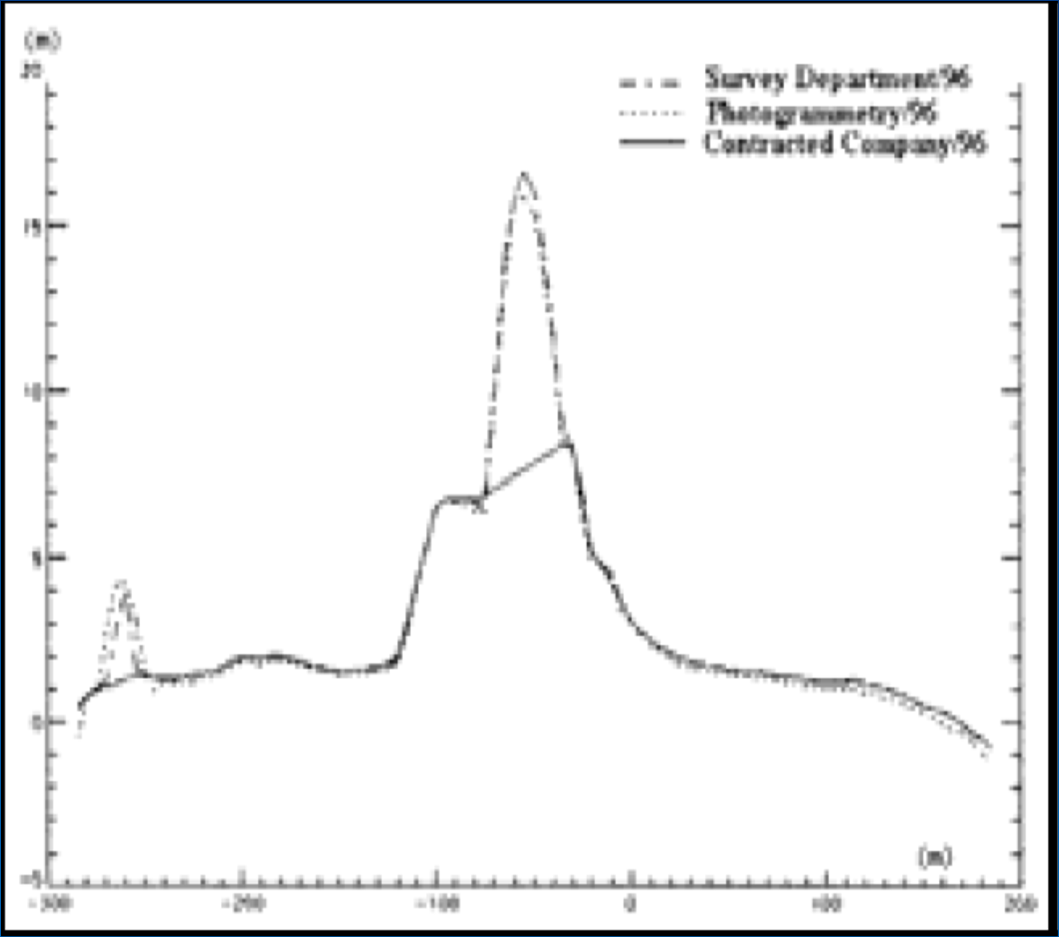
\includegraphics[width=0.5\linewidth]{figure/Chapter8/参照现有的高程数据}
	\caption{参照现有的高程数据}
	\label{fig:参照现有的高程数据}
\end{figure}

\paragraph{参照已有的地形图}如图\ref{fig:参照已有的地形图},地形图精度为10 cm,LiDAR影像的精度即每像素大小25 cm。
\begin{figure}[htbp]
	\centering
	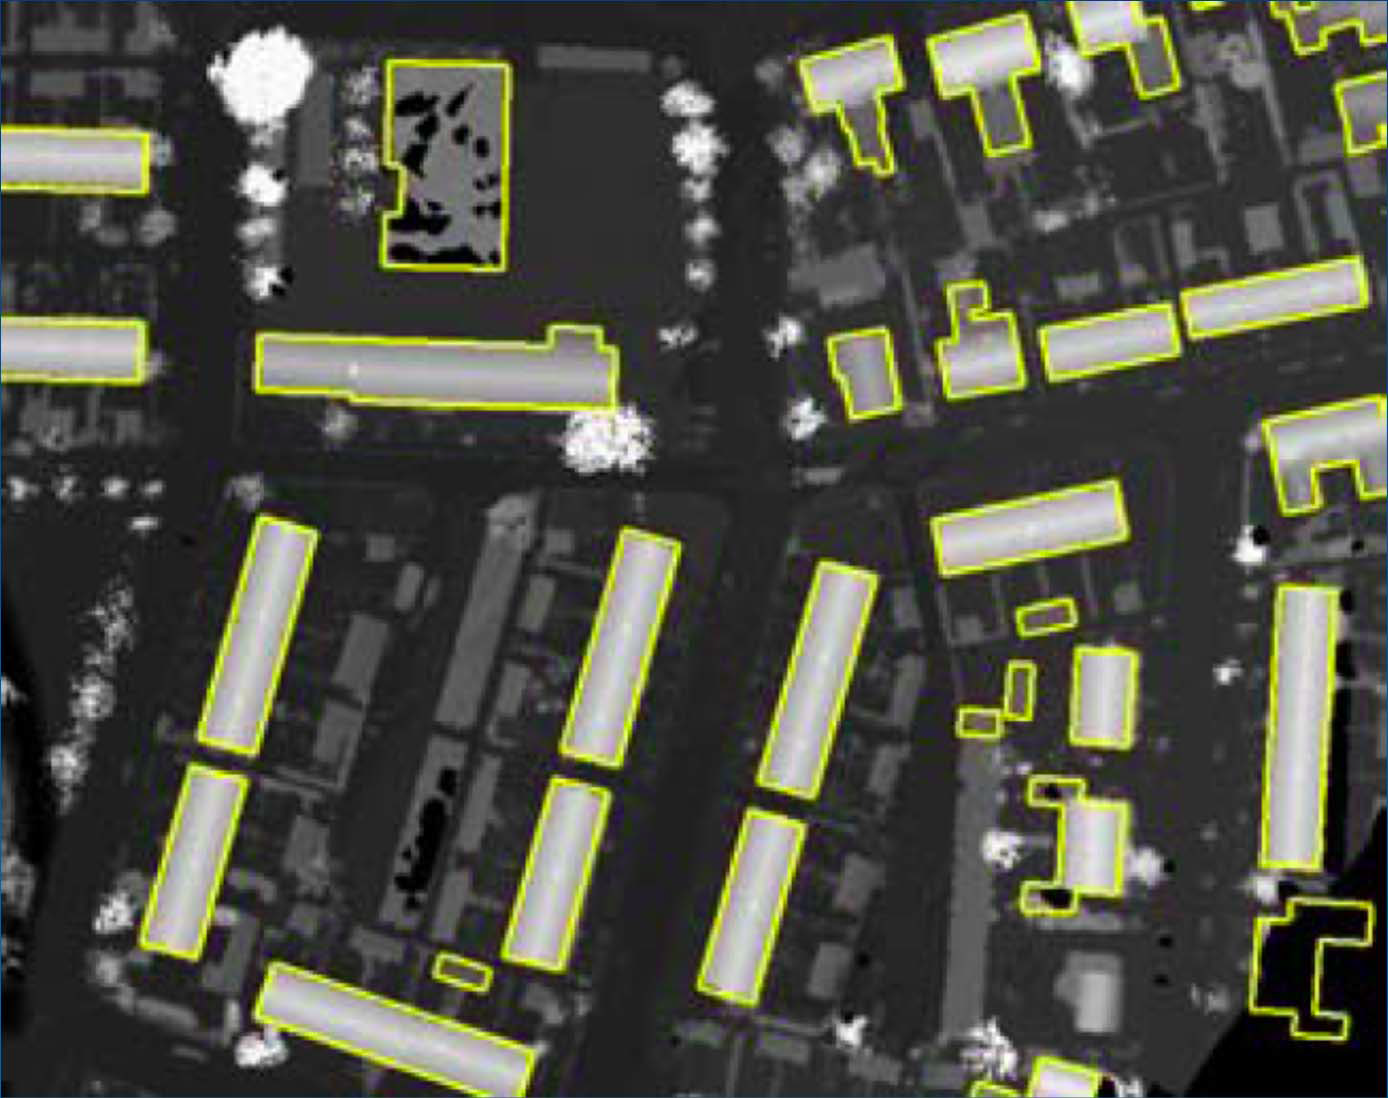
\includegraphics[width=0.6\linewidth]{figure/Chapter8/参照已有的地形图}
	\caption{参照已有的地形图}
	\label{fig:参照已有的地形图}
\end{figure}
